%----------------------------------------------------------------
%
%  File    :  survey-responsive-tables.tex
%
%  Author  :  Mirza Kabiljagic, Stefan Rajinovic, Aleksandar Stojicic,
%             Inti Gabriel Mendoza Estrada
%
%  Created :  27 May 20xx
%
%  Changed :  05 Dec 2019
%
%----------------------------------------------------------------

\chapter{Responsive Tables}
\label{chap:respt}

Due to the increasing amount of screens and their varying shapes,
sizes, and developers' space allocation when designing and
implementing tables, responsive table techniques have been `developed'
by manipulating the table's columns and rows to provide an optimal
experience for users across most mediums. It means the row and columns
can be repositioned, resized, collapsed, minimized, etc..

Data tables can contain many information, which makes displaying that
data quite messy and hard to look at. So by using responsive design, a
big favor is done to the clients, by adjusting the table according to
their devices. One idea would be to minimize the table, but if the
user is looking at the table from his mobile device, he would have to
zoom in, which is not that useful to him, because then again he would
need to scroll to view the whole table \parencite{Alligator}.

\begin{figure}[tp]
    \centering

    {%
    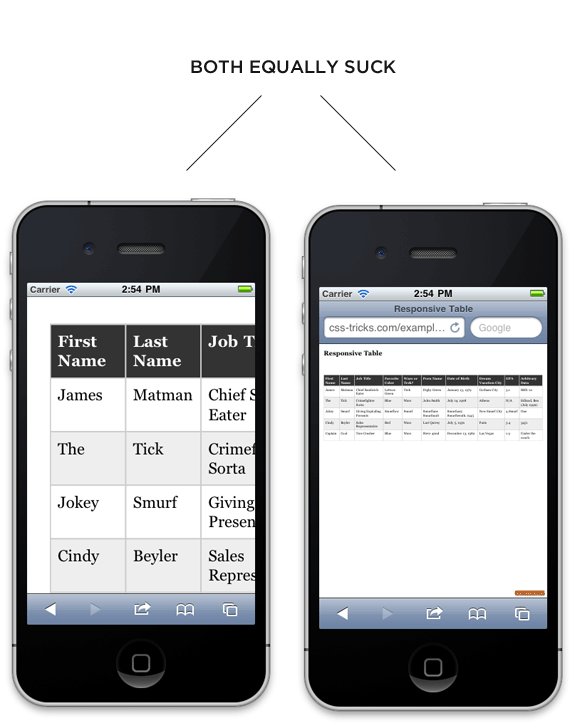
\includegraphics[width=0.30\linewidth]
    {images/zoom_1.png}%
    \label{zoom_1}%
    }


    \caption[Before reponsive]
    {

    \imgcredit{https://css-tricks.com/responsive-data-tables/.}
    }
    \label{fig:before_responsive}
\end{figure}

As seen in Figure \ref{fig:before_responsive}, both options do not really look nor
perform well. So, by using some simple CSS it is possible to fix that
problem. With the help of the mentioned media queries, it is possible
to specify for which device sizes, which settings should be used.

\begin{lstlisting}[%
    float=tp,
    language = CSS,
    xleftmargin=0cm,              % no extra margins for floats
    xrightmargin=0cm,             % no extra margins for floats
    language=biblatex,
    basicstyle=\footnotesize\ttfamily,
    frame=shadowbox,
    numbers=left,
    label=list:mediaq_on_table,
     stringstyle=\color{blue}
    ,
]
% An example of using simple CSS with media queries on how to 
% achieve Responsive Design:

@media
only screen and (max-width: 760px),
(min-device-width: 768px) and (max-device-width: 1024px)  {

  /* Force table to not be like tables anymore */
  table, thead, tbody, th, td, tr {
    display: block;
  }

  /* Hide table headers (but not display: none;, for accessibility) */
  thead tr {
    position: absolute;
    top: -624.9375rem;
    left: -624.9375rem;
  }

  tr { border: 0.0625rem solid #ccc; }

  td {
    /* Behave  like a "row" */
    border: none;
    border-bottom: 0.0625rem solid #eee;
    position: relative;
    padding-left: 50%;
  }

  td:before {
    /* Now like a table header */
    position: absolute;
    /* Top/left values mimic padding */
    top: 0;
    left: 0.375rem;
    width: 45%;
    padding-right: 0.625rem;
    white-space: nowrap;
  }
}
\end{lstlisting}

And now, the end result is seen in the Figure \ref{fig:figZoom3}.
\begin{figure}[tp]
    \centering

    {%
    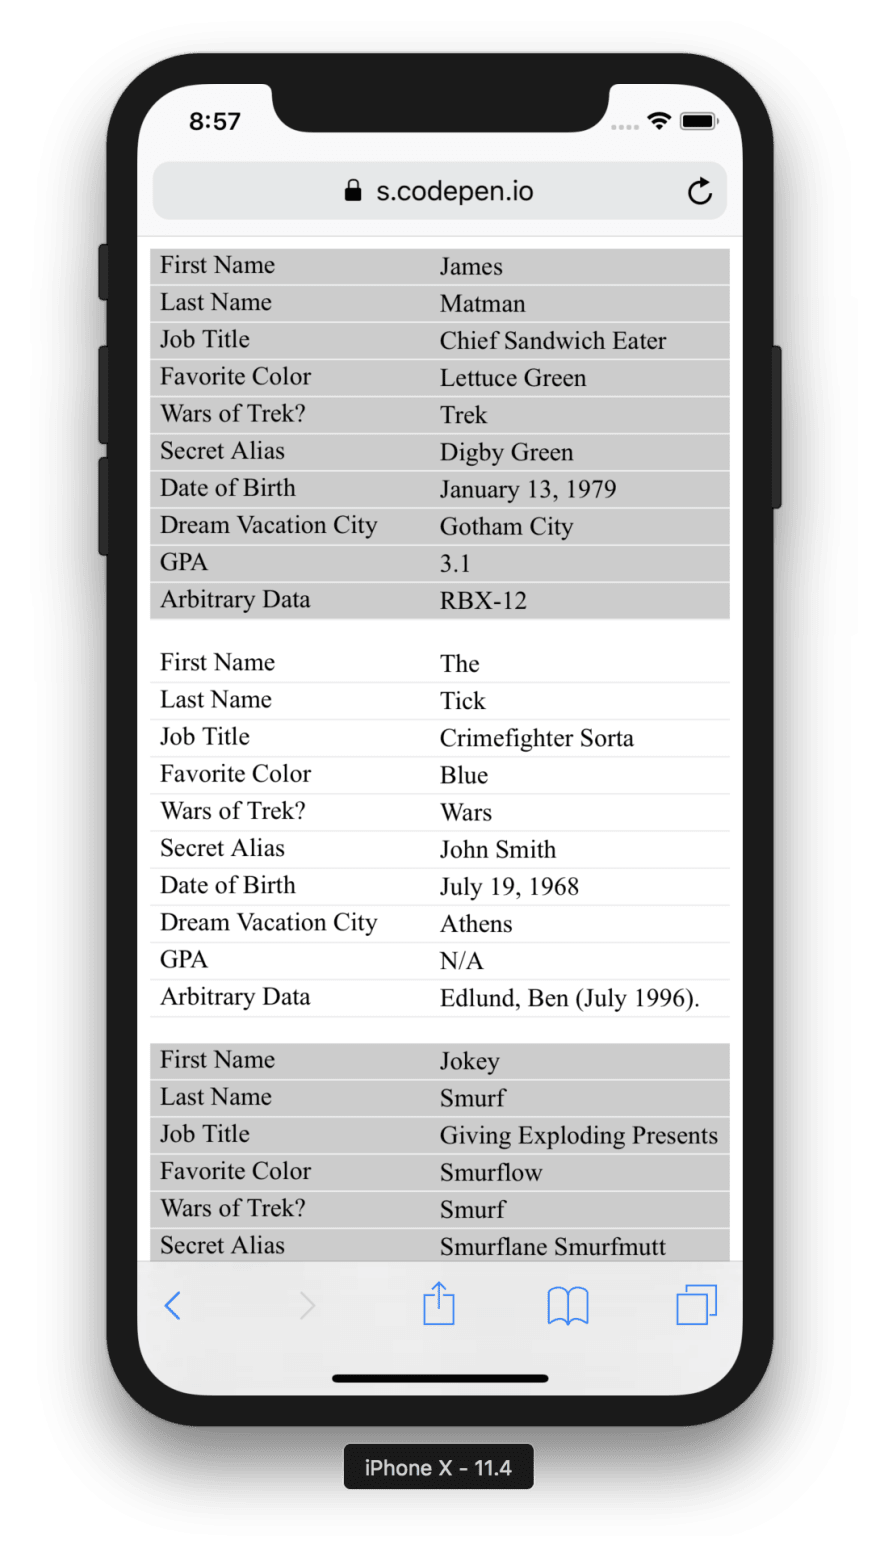
\includegraphics[width=0.45\linewidth]
    {images/zoom_3.png}%
    \label{zoom_3}%
    }


    \caption[After reposnsive]
    {

    \imgcredit{https://css-tricks.com/responsive-data-tables/.}
    }
    \label{fig:figZoom3}
\end{figure}


Some of the most popular responsive techniques are:
\begin{itemize}
    \item[--] Hidden Columns - Selected by User
    \item[--] Horizontal Scroll
    \item[--] Fixed Header
    \item[--] Flip Scroll
    \item[--] User Resizeable Columns
    \item[--] Long Two Column
\end{itemize}

In the following sections we will try to give a brief but detailed
description of what exactly each technique consists of, as well as the
reason to include this techniques on tables, and the code required to
implement such techniques.

\section{Horizontal Scroll}
When the allocated space is too small - horizontally, instead of
hiding it, a horizontal scroll bar (just for the table) is created.
The user can then scroll away.

Horizontal Scrolling represents a technique that resizes the table
into columns at small screen resoultion \parencite{HS_1}. 
This is different from viewport scrolling as we scroll only through 
the table.

It is very useful technique when presenting large data
 sets with identifiers in the first column. Then is very easy for 
 every user to compare data content with 
 multiple identifiers\parencite{HS}.

This solution works for following browsers:
\begin{itemize}
    \item[--] Google Chrome
    \item[--] Mozzila Firefox
    \item[--] Internet Explorer
    \item[--] Opera
    \item[--] Microsoft Edge
\end{itemize}

It is impossible to find one size that fits all solution. Data 
comparing is very difficult on the small screens.
There are a lot of possible workarounds for this issue, but no 
one can solve this problem \parencite{HS_1}.
Our implementation of horizontal scrolling creates table elements
 scrollable, but also can not solve the issue 
 to the end\parencite{HS_1}.

The code required to implement this technique 
on a table is shown in Listing \ref{list:HScroll}.

\begin{lstlisting}[%
    float=tp,
    language = CSS,
    xleftmargin=0cm,              % no extra margins for floats
    xrightmargin=0cm,             % no extra margins for floats
    language=biblatex,
    basicstyle=\footnotesize\ttfamily,
    frame=shadowbox,
    numbers=left,
    label=list:HScroll,
     stringstyle=\color{blue}
    ,
]
.rtable {
  display: inline-block;
  vertical-align: top;
  max-width: 100%;

  overflow-x: auto;

  // optional - looks better for small cell values
  white-space: nowrap;

  border-collapse: collapse;
  border-spacing: 0;
}

\end{lstlisting}

This CSS code represents CSS class \propname{.rtable} used in the case
when container is not resized. With display: inline-block all items
are listed horizontally instead of vertically. \propname{vertical-align} 
property maintains how elements set next to each other in a line. The 
\propname{overflow} property determines whether to crop content or
to add scroll bars (along the x-axis) when a table's content is too
big to satisfy some screen resolution. We can use \propname{white-space: nowrap} 
property as optional for small cell values. CSS border properties are used 
to control borders into a table\parencite{HS_1}.

An example HTML table with this technique is shown in Figure \ref{fig:horiz_scroll}.
\begin{figure}[tp]
    \centering

    {%
    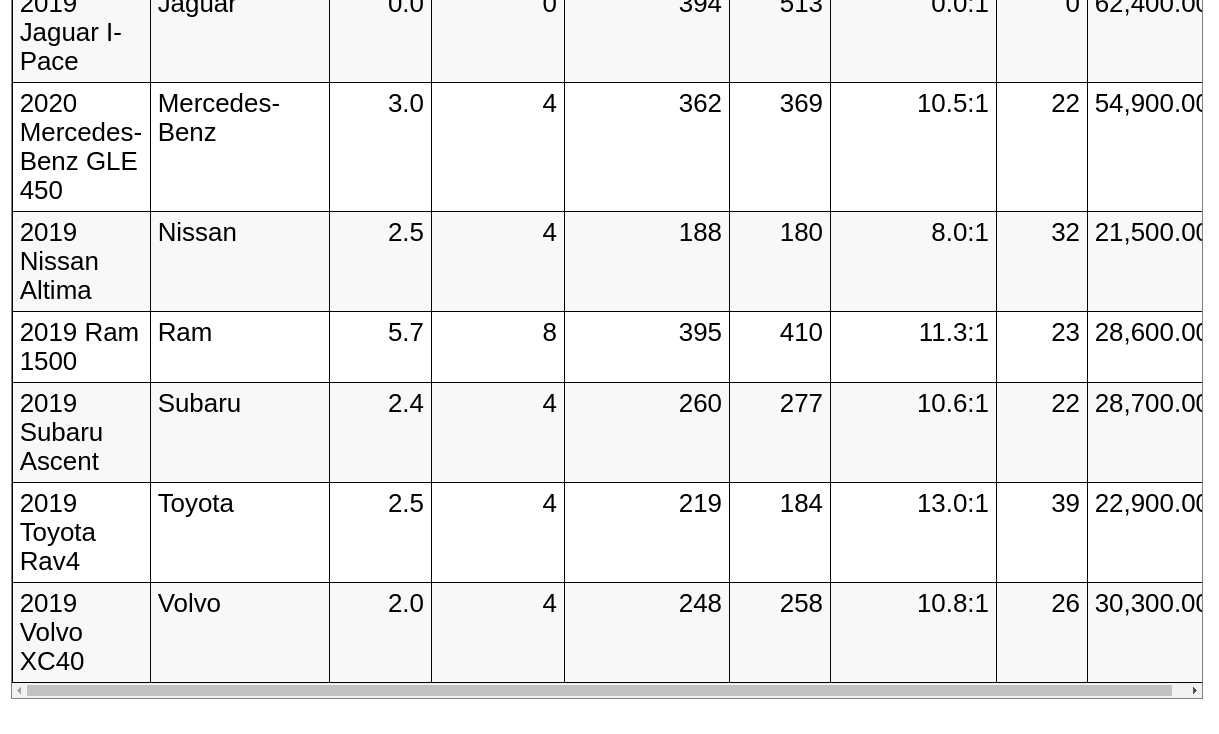
\includegraphics[width=1\linewidth]
    {images/horizontal.png}%
    \label{horizontal}%
    }


    \caption[Horizontal Scroll]
    {

    \imgcredit{Screenshot taken by the author.}
    }
    \label{fig:horiz_scroll}
\end{figure}

\section{Fixed Header}
When the table is vertically long, the table's header is fixed to the
top of the table's view. As we scroll down, the table's header is kept
always visible. It is very useful to have the fixed header (first row containing the
header cells) fixed on the top of the table, when presenting tables
with a particularly larage data set. This helps users to quickly
determine what every column identify rather than need to scroll back
to the top of the table every time.

Fixed Header provides information that allows the user to always know
in what column the cell the user is looking at is in. This is very effective feature 
that makes our life easier \parencite{HS}. An implementation can be seen in Listing
\ref{list:FixedHeader2}. This solution works for following browsers:
\begin{itemize}
    \item[--] Google Chrome
    \item[--] Mozzila Firefox
    \item[--] Internet Explorer
    \item[--] Opera
    \item[--] Microsoft Edge
\end{itemize}

\begin{lstlisting}[%
    float=tp,
    language = CSS,
    xleftmargin=0cm,              % no extra margins for floats
    xrightmargin=0cm,             % no extra margins for floats
    language=biblatex,
    basicstyle=\footnotesize\ttfamily,
    frame=shadowbox,
    numbers=left,
    label=list:FixedHeader2,
     stringstyle=\color{blue}
    ,
]
.fixedHeader tbody {
  display: block;
  overflow: auto;
  width: 100%;
}

.fixedHeader thead tr {
  display: table;
  width: 100%;
  table-layout: fixed;
}

.fixedHeader thead, .fixedHeader tbody tr {
  display: table;
  width: 100%;
  table-layout: fixed;
}

.fixedHeader thead {
  width: calc( 100% - 0.6em )
}

.fixedHeader td {
  width: 100%;
}

\end{lstlisting}

$<$\propname{tbody}$>$ element is determined with the type of rendering
box. With \propname{overflow: auto}, a scrollbar will appear along y-axis.
All $<$\propname{thead}$>$ and $<$\propname{tbody}$>$ rows will behave as
table elements. Fixed table layout algorithm is used to control table and column
widths. Width for almost every table element is static, just the header has
non-static width \parencite{FH_1}. The width of header is determined with 
the \propname{calc()} function to allow responsiveness \parencite{FH}.

An example HTML table with this technique is shown in Figure \ref{fig:fixed_header2}.

\begin{figure}[tp]
    \centering

    {%
    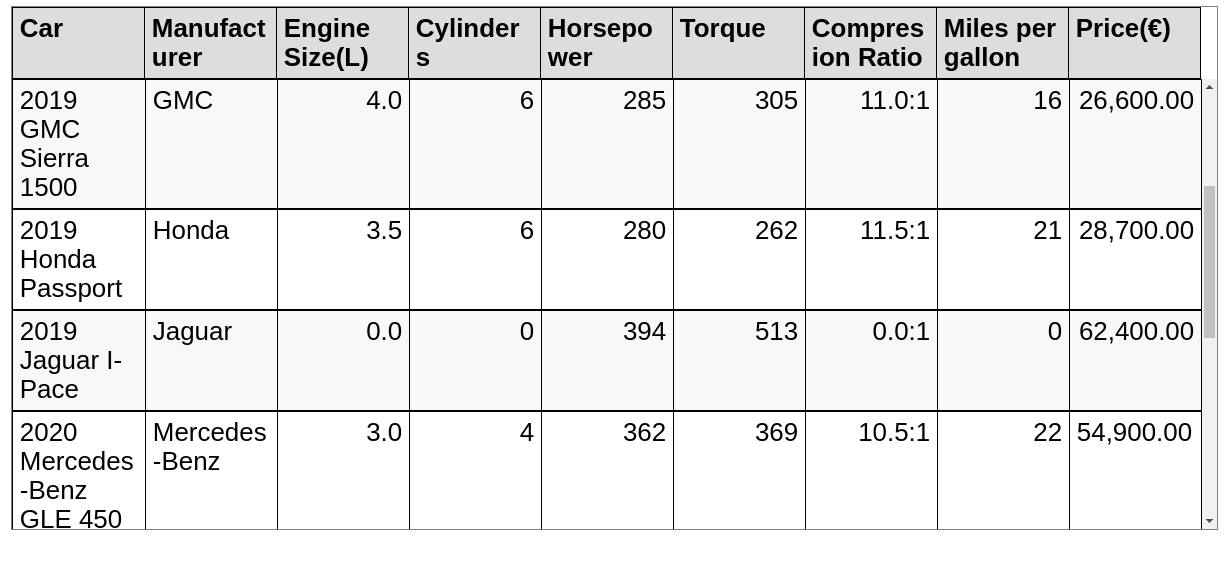
\includegraphics[width=1\linewidth]
    {images/fixed_header.png}%
    \label{fixed_header}%
    } 


    \caption[Fixed Header]
    { 

    \imgcredit{Screenshot taken by the author.}
    }
    \label{fig:fixed_header2}
\end{figure}

 
\section{Flip Scroll}
This technique is useful for an object-based table; one where each row
is populated by a single `object' where each column represents a
different feature of the object. If all features -- columns -- cannot
be seen at once, it is sometimes more desireable to be able to show
all features of an object rather than a good amount of (incomplete)
features for a good amount of objects.
\newline

Rather than having the user scroll through features, the user is now
able to scroll through objects horizontally instead. This is the
result of transposing the table. The first column will now house the
(previously column) headers and each column will be devoted to an
object, rather than each row. Flip scroll also `promises' to keep the 
table in the allocated space -- by allowing table horizontal scrolling.

An implementation can bee seen in Listing \ref{list:FlipScroll}. This 
solution works for following browsers:
\begin{itemize}
    \item[--] Google Chrome
    \item[--] Mozzila Firefox
    \item[--] Internet Explorer
    \item[--] Opera
    \item[--] Microsoft Edge
\end{itemize}

\begin{lstlisting}[%
    float=tp,
    language = CSS,
    xleftmargin=0cm,              % no extra margins for floats
    xrightmargin=0cm,             % no extra margins for floats
    language=biblatex,
    basicstyle=\footnotesize\ttfamily,
    frame=shadowbox,
    numbers=left,
    label=list:FlipScroll,
     stringstyle=\color{blue}
    ,
]
table.flipscroll{
  width: 100%;
  overflow-x: auto;
}
  
table.flipscroll  tbody tr { 
  display: inline-block; 
  vertical-align: top; 
}
  
table.flipscroll  tbody { 
  display: block; 
  width: auto; 
  position: relative; 
  overflow-x: auto; 
  white-space: nowrap; 
}
\end{lstlisting}

Setting \propname{width: 100\%} and \propname{overflow-x: auto} makes the
table horizontally scrollable and stick to the allocated space. The trick 
is setting the attribute \propname{display: inline-block} on the 
\propname{tbody tr} HTML tag and \propname{white-space: nowrap} on the
\propname{tbody} HTML tag \parencite{FS}.

Figure \ref{fig:FlipScroll} represents an HTML table with Flip Scroll.

\begin{figure}[tp]
    \centering

    {%
    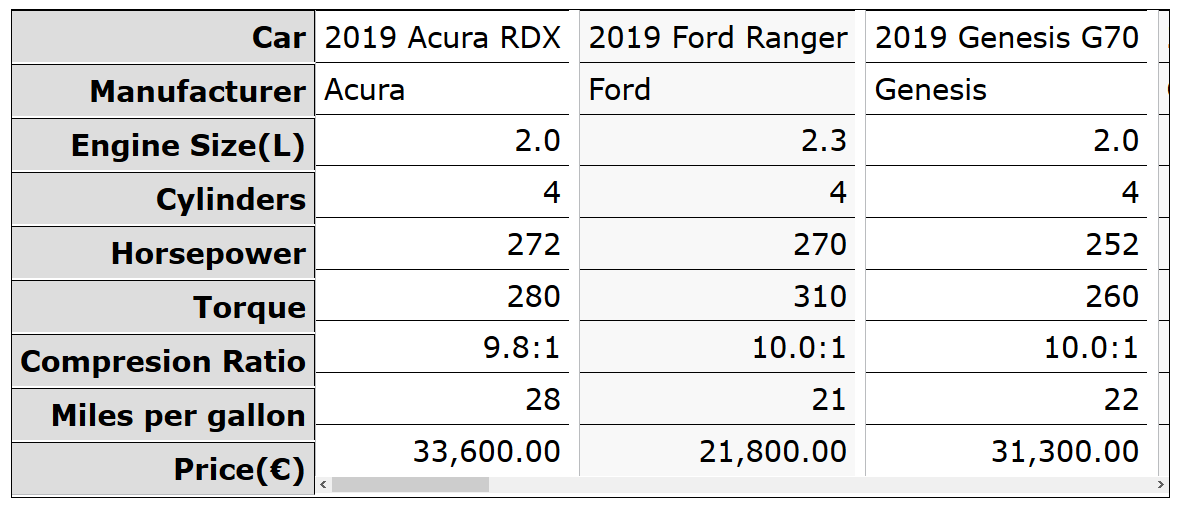
\includegraphics[width=1\linewidth]
    {images/flip_scroll.png}%
    \label{flip_scroll}%
    }


    \caption[Flip Scroll]
    {

    \imgcredit{Screenshot taken by the author.}
    }
    \label{fig:FlipScroll}
\end{figure}


\section{User Resizeable Columns}
This technique empowers the user quite significantly. As the title
suggests, the user is able to manipulate the size of a table's
columns. 

This technique is useful when the user is immune to space limitation
penalties the table might have on most other users. For example, if a
user has a screen big enough that space between columns is wasted to
keep column sizes consistent, being able to resize this column to
bring other columns into view is highly desireable.

User Resizeable Columns allows the user to tailor the table's
experience to his/her own preferences. There are two possible solutions. 
The solution using only CSS can be seen in Listings \ref{list:UserRColumns} 
and the solution using JQuery can be seen in Listing \ref{list:URC2}. 
Both work for following browsers:
\begin{itemize}
    \item[--] Google Chrome
    \item[--] Mozzila Firefox
    \item[--] Internet Explorer
    \item[--] Opera
    \item[--] Microsoft Edge
\end{itemize}

\begin{lstlisting}[%
    float=tp,
    language = CSS,
    xleftmargin=0cm,              % no extra margins for floats
    xrightmargin=0cm,             % no extra margins for floats
    language=biblatex,
    basicstyle=\footnotesize\ttfamily,
    frame=shadowbox,
    numbers=left,
    label=list:UserRColumns,
     stringstyle=\color{blue}
    ,
]
<thead>
    <tr>
        <th title="Car">
            <div class = "resizecell">Car</div>
        </th>
        <th title="Manufacturer">
            <div class = "resizecell">Manufacturer</div>
        </th>
        <th title="Engine Size(L)">
            <div class = "resizecell">Engine Size(L)</div>
        </th>
        [...]
    </tr>

</thead>
  .resizecell {
    resize: horizontal;
    overflow: auto;
    width: 100%;
    hyphens: auto;
  }
<style>

</style>
\end{lstlisting}

Encapsulating every header cell (or every single cell) with a
\propname{$<$div$>$} tag allows CSS to enable resizeability by setting
the attribute \propname{resize: horizontal} to these divs
\parencite{URC_1}.

Figure \ref{fig:URCCSS} represents an HTML table with User Resizeable Columns
using only HTML and CSS.

\begin{figure}[tp]
    \centering

    {%
    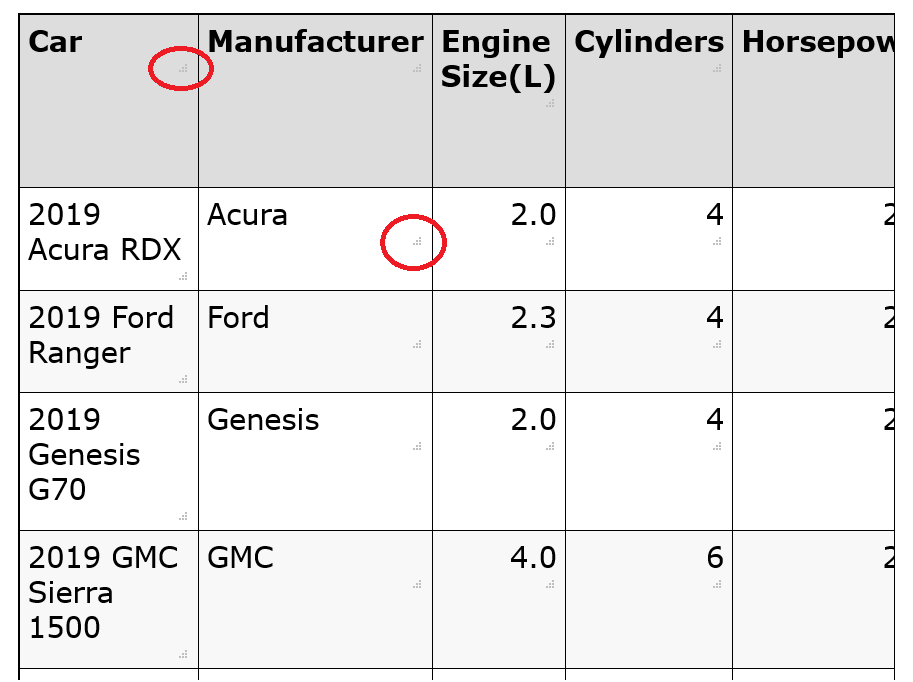
\includegraphics[width=1\linewidth]
    {images/urc_css.png}%
    \label{urc_css}%
    }


    \caption[User Resizeable Columns using only HTML and CSS]
    {

    \imgcredit{Screenshot taken by the author.}
    }
    \label{fig:URCCSS}
\end{figure}

\begin{lstlisting}[%
    float=tp,
    language = CSS,
    xleftmargin=0cm,              % no extra margins for floats
    xrightmargin=0cm,             % no extra margins for floats
    language=biblatex,
    basicstyle=\footnotesize\ttfamily,
    frame=shadowbox,
    numbers=left,
    label=list:URC2,
    stringstyle=\color{blue},
]
~/js/jQuery.resizableColumns.js

$(function(){
  $('.rcl').resizeableColumns();
}); 
\end{lstlisting}

The trick to use this technique using JQuery is calling the 
\propname{resizeableColumns()} on the table of your choice \parencite{URC_2}.
The resulting image can be seen in Figure \ref{fig:URCJS}.

\begin{figure}[tp]
    \centering

    {%
    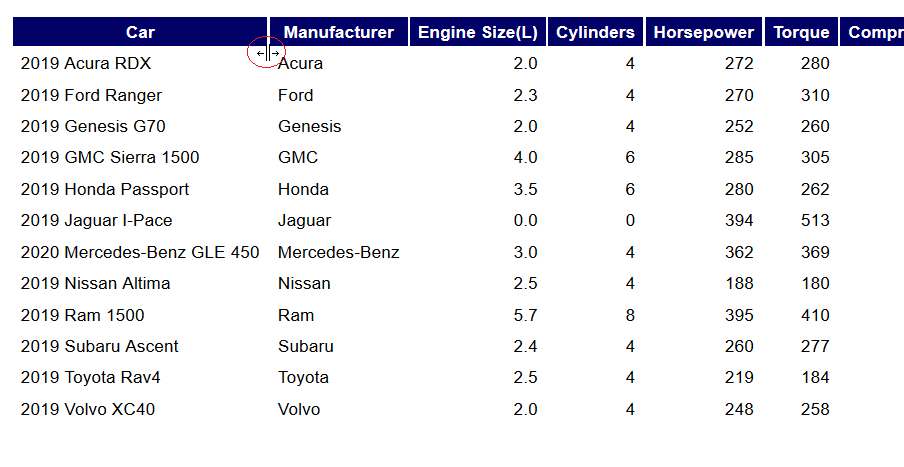
\includegraphics[width=1\linewidth]
    {images/urc_js.png}%
    \label{urc_js}%
    }


    \caption[User Resizeable Columns using JS (jQuery)]
    {

    \imgcredit{Screenshot taken by the author.}
    }
    \label{fig:URCJS}
\end{figure}

\section{Long Two Column}
Just like Flip Scroll, this technique is useful for an object-based
table; one where each row is populated by a single `object' where each
column represents a different feature of the object. 

Rather than having the user scroll through features, the user is now
able to scroll through objects vertically instead. This is the result
of transposing the table. The first column will now house the
(previously column) headers and the second column will house the data
previously housed in the first row. This creates a `minitable' for the
(previously) first row. For the next object (and row), another
`minitable' is created like with the first one and then appended
below. This approach creates a `minitable' for each object and appends
it to the previous object. 

As the name suggest, you end up with a long table of 2 columns, the
first of which is 'always the same'. Unlike Flip scroll, it does not 
keep the table in the allocated space, unless you set vertical scrolling.
This solution works for following browsers:\begin{itemize}
    \item[--] Google Chrome
    \item[--] Mozzila Firefox
    \item[--] Internet Explorer
    \item[--] Opera
    \item[--] Microsoft Edge
\end{itemize}

\begin{lstlisting}[%
    float=tp,
    language = CSS,
    xleftmargin=0cm,              % no extra margins for floats
    xrightmargin=0cm,             % no extra margins for floats
    language=biblatex,
    basicstyle=\footnotesize\ttfamily,
    frame=shadowbox,
    numbers=left,
    label=list:LongTwoColumn,
     stringstyle=\color{blue}
    ,
]
table, thead, tbody, th, td, tr {
  display: block;
}

td {
  /* Behave  like a "row" */
  border: none;
  border-bottom: 0.0625rem solid #eee;
  position: relative;
  padding-left: 50%;
}

td:before {
  /* Now like a table header */
  position: absolute;
  /* Top/left values mimic padding */
  top: 0;
  left: 0.375rem;
  width: 45%;
  padding-right: 0.625rem;
  white-space: nowrap;
}
\end{lstlisting}

As seen in Listing \ref{list:LongTwoColumn}, trick is setting the 
table's elements to \propname{display: block} and the $<$\propname{td}$>$ 
 tag's attribute to \propname{position: relative} \parencite{L2C}.
 Figure \ref{fig:LongTwoColumn} shows an HTML table with Long Two Column
 technique applied to it.

\begin{figure}[tp]
    \centering

    {%
    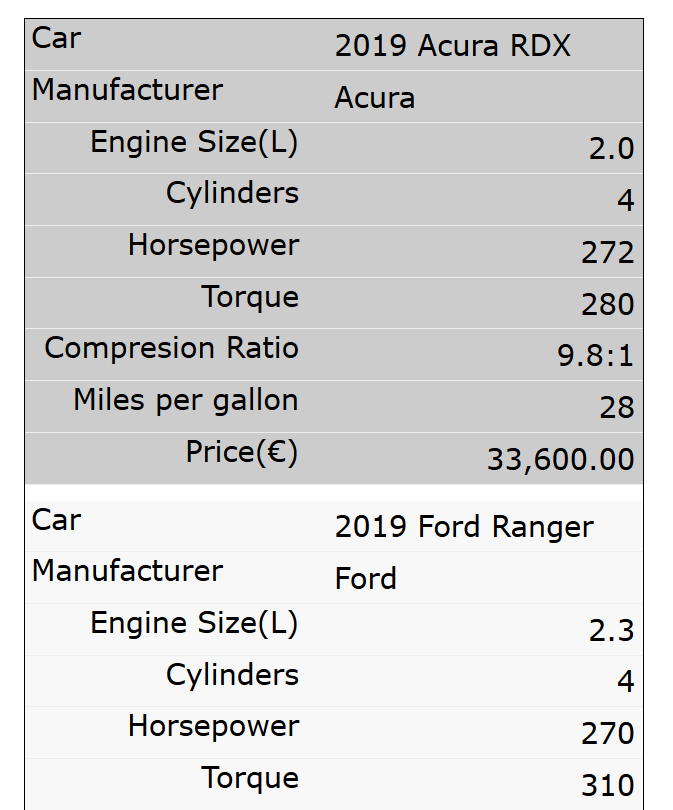
\includegraphics[width=0.5\linewidth]
    {images/long_two_column.png}%
    \label{long_two_column}%
    }


    \caption[Long Two Column] 
    {

    \imgcredit{Screenshot taken by the author.}
    }
    \label{fig:LongTwoColumn}
\end{figure}
